        \documentclass{standalone}
        \usepackage{tikz}
        \begin{document}
        \fontsize{16px}{16px}\selectfont
        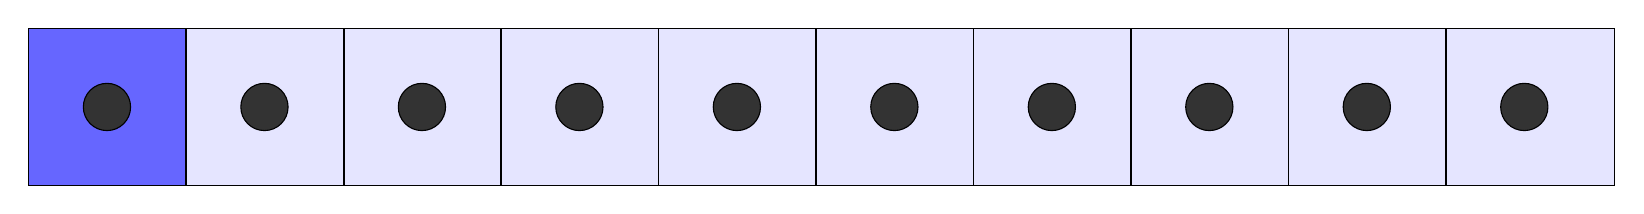
\begin{tikzpicture}
[scale=1]
\fill[blue!60!white, draw=black] (0,0) rectangle (2,2);
\fill[black!80!white, draw=black] (1,1) circle (0.3cm);
\fill[blue!10!white, draw=black] (2.01,0) rectangle (4,2);
\fill[black!80!white, draw=black] (3,1) circle (0.3cm);
\fill[blue!10!white, draw=black] (4.01,0) rectangle (6,2);
\fill[black!80!white, draw=black] (5,1) circle (0.3cm);
\fill[blue!10!white, draw=black] (6.01,0) rectangle (8,2);
\fill[black!80!white, draw=black] (7,1) circle (0.3cm);
\fill[blue!10!white, draw=black] (8.01,0) rectangle (10,2);
\fill[black!80!white, draw=black] (9,1) circle (0.3cm);
\fill[blue!10!white, draw=black] (10.01,0) rectangle (12,2);
\fill[black!80!white, draw=black] (11,1) circle (0.3cm);
\fill[blue!10!white, draw=black] (12.01,0) rectangle (14,2);
\fill[black!80!white, draw=black] (13,1) circle (0.3cm);
\fill[blue!10!white, draw=black] (14.01,0) rectangle (16,2);
\fill[black!80!white, draw=black] (15,1) circle (0.3cm);
\fill[blue!10!white, draw=black] (16.01,0) rectangle (18,2);
\fill[black!80!white, draw=black] (17,1) circle (0.3cm);
\fill[blue!10!white, draw=black] (18.01,0) rectangle (20.15,2);
\fill[black!80!white, draw=black] (19,1) circle (0.3cm);
        \end{tikzpicture}
        \end{document}
